Ici, nous avons ajouté la contrainte de l'intégralité des variables dans le solveur, ce qui a pour effet de modifier légèrement la courbe, tout en gardant les caractéristiques importantes observées à la question précédente.

\begin{figure}[H]
    \centering
    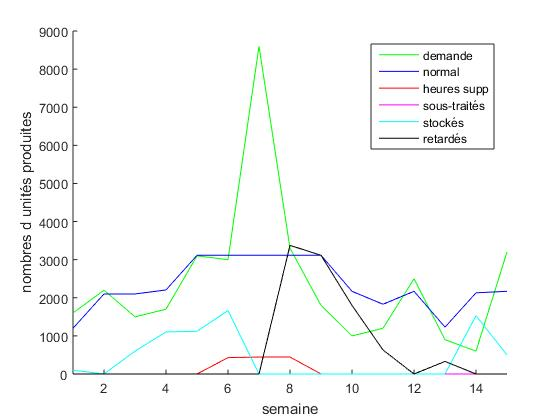
\includegraphics[width=0.8\textwidth]{graphes/graphq9.jpg}
    \caption{Graphe de la production à personnel variable entier}
    \label{fig:q8_01}
\end{figure}

\begin{figure}[H]
    \centering
    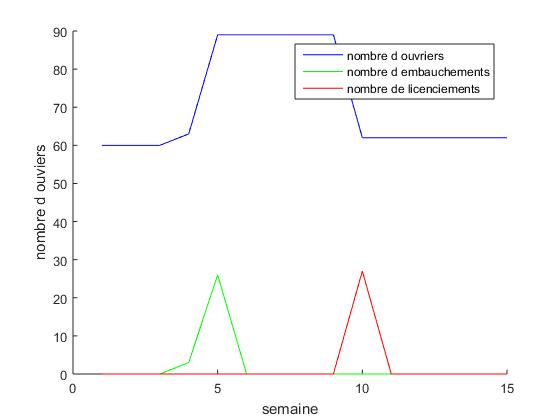
\includegraphics[width=0.8\textwidth]{graphes/ouvrierq9.jpg}
    \caption{Graphe de la variation du personnel entier}
    \label{fig:q8_02}
\end{figure}
